% Chapter 6
\chapter{Advertisement High Fidelity prototype} % Main chapter title

\label{Chapter6} % For referencing the chapter elsewhere, use \ref{Chapter1} 

\newpage

\section{Introduction}
A follow up study is conducted when a final version of a prototype is ready. A \emph{summative} ``\emph{is used to evaluate how well the design meets the usability requirements}''\cite{summative}. It is to finalize the decisions on a prototype, there have been studies like ``\emph{Sweep and point \& shoot}'' \cite{SweepPointShoot} that evaluated prototypes for interaction of personal computing device with large public displays. Another evaluation was of ``\emph{mobile interaction with live video}'' \cite{TouchProjector} that used a with-in subject design, where the participant’s performance were measured for automatic zooming and temporary image freezing. Sebastian .D \cite{WalldragandDrop} assessed the general performance of drag and drop interaction on large displays and compared it with a traditional drag and drop. Jorg Müller \cite{LookingGlass} did pre-studies (lab and field) on noticing interactivity of a display in which the time required for recognizing interactivity by participants were measured.

Based on the feedbacks from the low-fidelity evaluation in the previous chapter, I developed two functional hi-fidelity version of interactive advertisement of the body and mobile. This chapter explains the evaluation process of the Hi-fidelity prototypes of interactive advertisement both body and mobile. The evaluations were more on user performance, user acceptance and usability issues. As the application would be in public, where many people would interact, the application performance was also tested with single and multi-users to ensure application stability.


\section{Advertisement prototypes}
The prototype was to show a city map on the screen with possible interactive famous places of Bauhaus. The interaction idea was to map physical movement of the user, or map the cursor movement of a phone to the virtual movement on the city map. The interaction let users to explore the target places by reaching those locations. Five places were to be explored by one person to complete the interaction.


In this prototype there were mainly three hierarchical levels of interfaces, (1) \emph{Call-to-Action}, (2) \emph{Game interaction}, and (3) the advertisement video interface.

\begin{itemize}
\item \emph{Call-to-Action} interface: \\
This interface invites participants to interact with the application. This method was first proposed by Bill Kules \cite{call-to-action}, in which the immediate usability of public accesses to a system was designed. \emph{Call-to-Action} of body and mobile are designed differently, which are shown in below sections. 

\item Interaction interface: \\
This interface activates when the user follows the instructions of the first interface, the interface shows the interactive map with the hotspots to be explored by participants.

\item Video advertisement: \\
After the interaction is completed then a silent video advertisement is shown for 20 seconds. 
The advertisement video was created in powtoon\footnote{Powtoon: \url{https://www.powtoon.com}, last accessed: 21 April 2016} with a free version account, to see the full advertisement video visit below these videos, video1\footnote{Old video version: \url{https://www.youtube.com/watch?v=GrWtOyjNcQ0}} and video2\footnote{ New video version: \url{https://www.youtube.com/watch?v=-y1Dbz6E6bU&feature=youtu.be}}

\end{itemize}


\newpage
\subsection{Body prototype}
This section introduces the interfaces of the body interactive prototype and the processes of how a user can start interaction. Watch this demo video\footnote{Body interaction: \url{https://www.youtube.com/watch?v=Uhvn43gImmk}, last accessed: 29 June 2016} to have a short glance to the interactions.

\begin{enumerate}

\item \emph{Call-to-Action} interface: \\
This interface is basically attraction attention and \emph{Call-to-Action}interface. As you can see below picture, there is someone standing in front of the screen and the interface calls the person to come near. This interface also has alert message section on the top right that alerts the participant if moved away from the camera range. 

\begin{figure}[H]
    \centering
    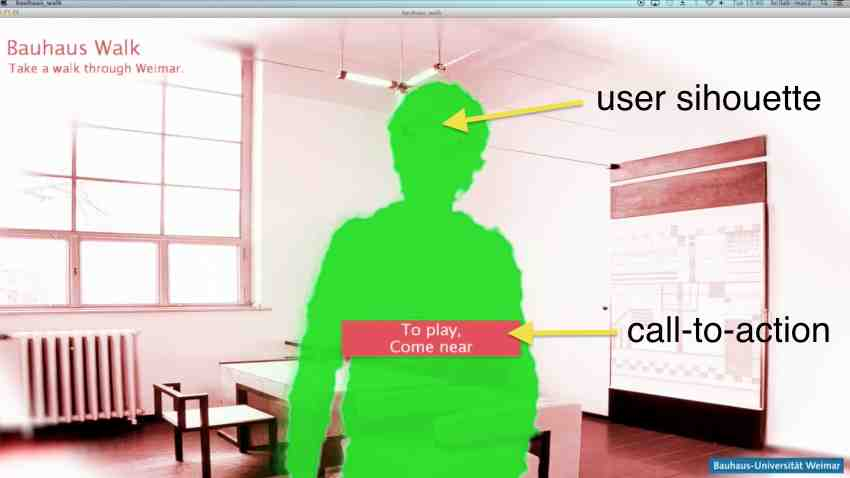
\includegraphics[width=120mm,height=70mm]{Figures/6/body/first_interface}
    \caption{call-to-action interface}%
    \label{fig:body_firstinterface}%
\end{figure}

When a new person steps in the range of the camera, his/her silhouette is projected on the screen with a different color, and then the application calls the person to come near in order to trigger the game.


\item Transition to interaction interfaces: \\
The transition happens when the person stands close to the screen for more than 3 seconds and the below things happen.

\begin{enumerate}
\item Loading animation:\\
 The loading animation is a reaction to the action of the participants, which gives the user a clue that the interaction will be started. 

\item Scaling down the silhouette: \\
The participant's silhouette is scaled down to allow him/her to walk freely on the map and to give the participant the feeling of walking, 

\item Show task instruction:  \\
Every interaction has an instruction, the instruction is fairly very easy and it is simplified in one sentence as, ``\emph{To play, come near}''.
\end{enumerate}

\begin{figure}[H]
    \centering
    \begin{subfigure}[H]{0.3\textwidth}
        \centering
        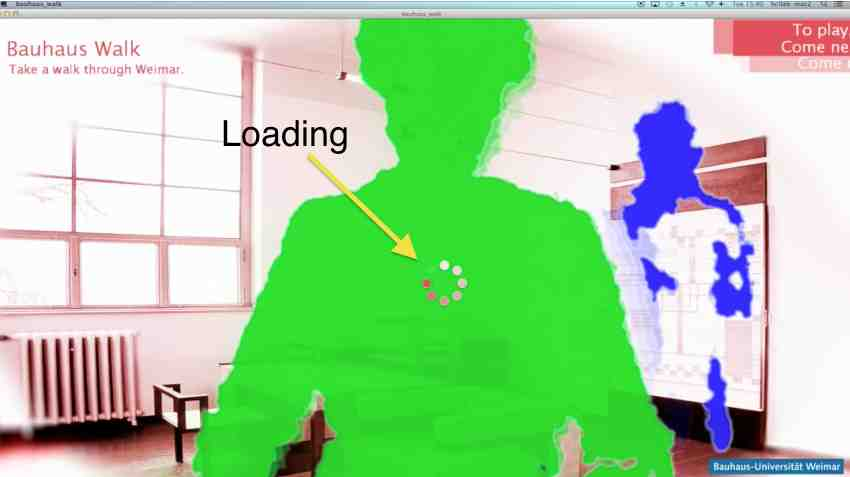
\includegraphics[width=\textwidth,height = 3.5cm]{Figures/6/body/loading}
        \caption{Loading}
        \label{fig:loading_logo}
    \end{subfigure}
    \begin{subfigure}[H]{0.3\textwidth}
        \centering
        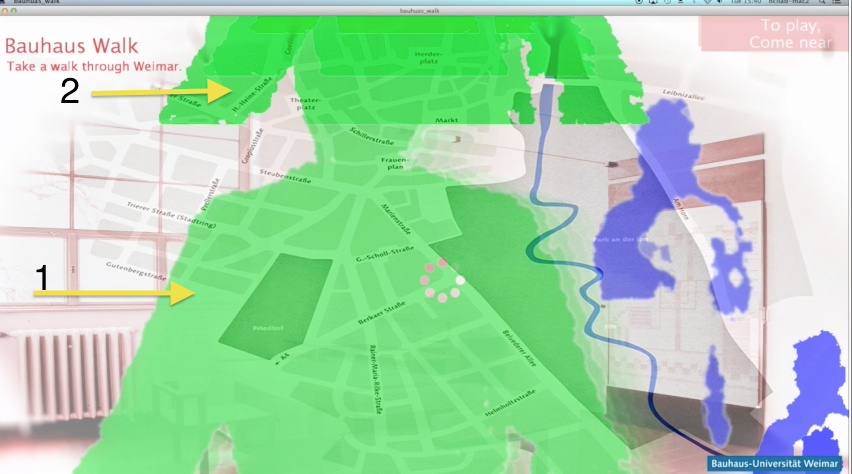
\includegraphics[width=\textwidth,height = 3.5cm]{Figures/6/body/scalling_down}
        \caption{Scalling down}
        \label{fig:scalling_down}
    \end{subfigure} 
      \begin{subfigure}[H]{0.3\textwidth}
        \centering
        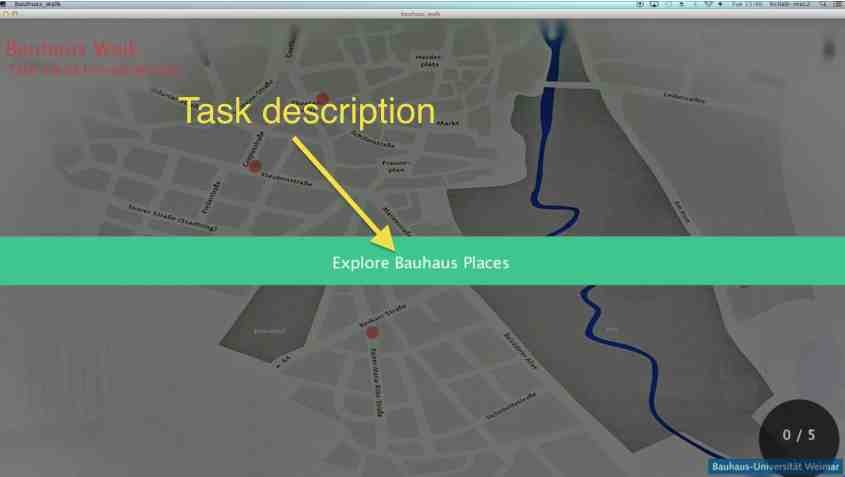
\includegraphics[width=\textwidth,height = 3.5cm]{Figures/6/body/task_description}
        \caption{Task description}
        \label{fig:task_description}
    \end{subfigure}
    \caption{Transitions of interfaces }
    \label{fig:transition_sequence}
\end{figure}


\item Interaction interface: \\
In this interface, participants can interact with the elements on the map. As shown in the picture below, the silhouette has visited four locations and has a score of 4 out of 5. In order to finish the interaction the user needs to visit the last location.

\begin{figure}[H]
    \centering
    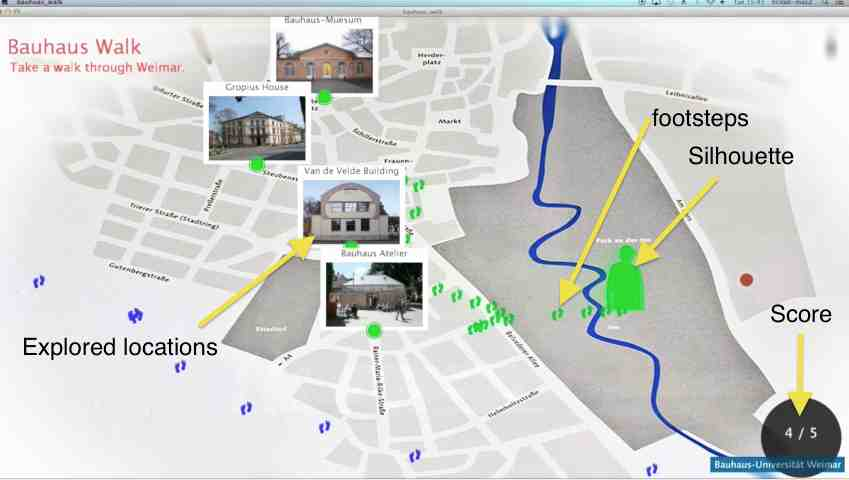
\includegraphics[width=130mm,height=80mm]{Figures/6/body/interaction_inter}
    \caption{Second Interface}%
    \label{fig:body_secondinterface}%
\end{figure}

%\subsubsection{Flowchart Diagram}
%The below chart roughly shows the flow of the application.
%\begin{figure}[H]
%    \centering
%    \includegraphics[width=120mm,height=140mm]{Figures/7/body_interactive/body_flow_chart}
%    \caption{Body Interactive advertisement Flowchart diagram}%
%    \label{fig:Body_flowchat}%
%\end{figure}

\end{enumerate}

\subsection{Mobile}
Mobile interaction is possible by using a smartphone and a Wi-Fi connection to the advertisement network. The user should open the mentioned IP address in his / her mobile browser and enter a name to login. After login, a mobile controller appears by which the user can control the map elements on the screen. Watch this demo video\footnote{Mobile interaction: \url{https://www.youtube.com/watch?v=ooxWjgd0xUs}, last accessed: 29 June 2016} to have a short glance to interactions.

\begin{enumerate}

\item \emph{Call-to-Action} interface: \\
This interface is designed in such a way to attract passersby and also guide the participants on how to use their smartphone to access the advertisement application. The attraction is again the same method that was used for the body, the passersby silhouette is projected at the back of the Access information. The interface has a QR code that could be easy to be scanned instead of typing the whole IP address. There is an alert area that gets activated when a person is logged in and has not changed the orientation of the phone to landscape.

\begin{figure}[H]
    \centering
    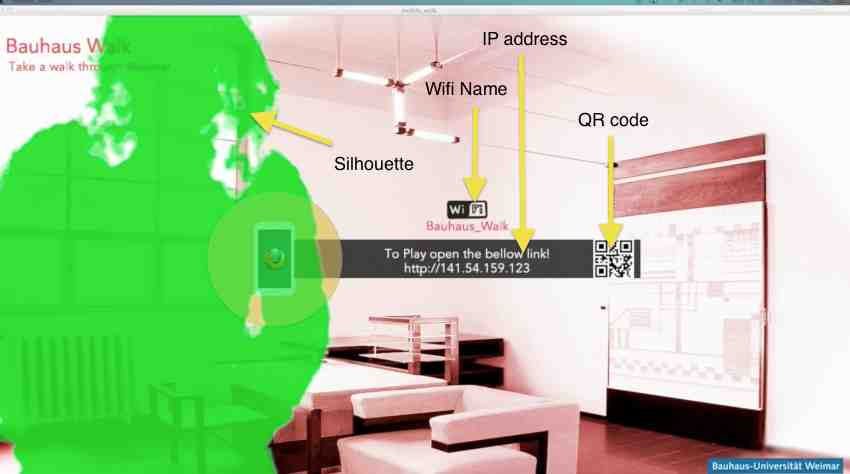
\includegraphics[width=120mm,height=70mm]{Figures/6/mobile/call-to-action}
    \caption{Mobile interactive interface:}%
    \label{fig:mobile_firstinterface}%
\end{figure}



\item Transition to interaction interfaces: \\
The transition happens only when the user connects to the Wi-Fi, open the controller and physically holds the phone in landscape.

\begin{enumerate}
\item Loading animation:\\
The loading animation is a reaction to the action of the participants, which gives the user a clue that the interaction will be started. 
\item  Creating Colored cursor: \\
A colored circle is created for the participant in the center of the screen. Each participant has different color matching to his/her controller interface in his or her phone.
\item Show task instruction:  \\
The instruction is fairly very easy and it is simplified in one sentence to explore locations on the map by using their phone.


\end{enumerate}


\begin{figure}[H]
    \centering
    \begin{subfigure}[H]{0.45\textwidth}
        \centering
        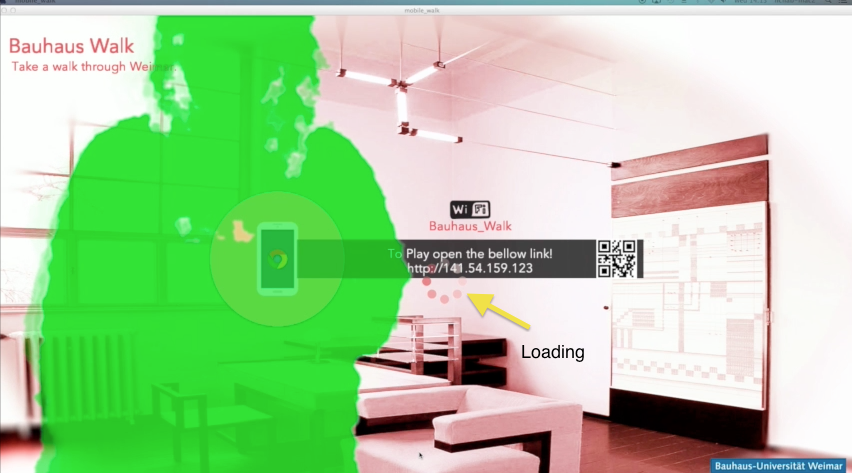
\includegraphics[width=\textwidth,height=4cm]{Figures/6/mobile/loading}
        \caption{Loading}
        \label{fig:loading_mobile}
    \end{subfigure}
    \begin{subfigure}[H]{0.45\textwidth}
        \centering
        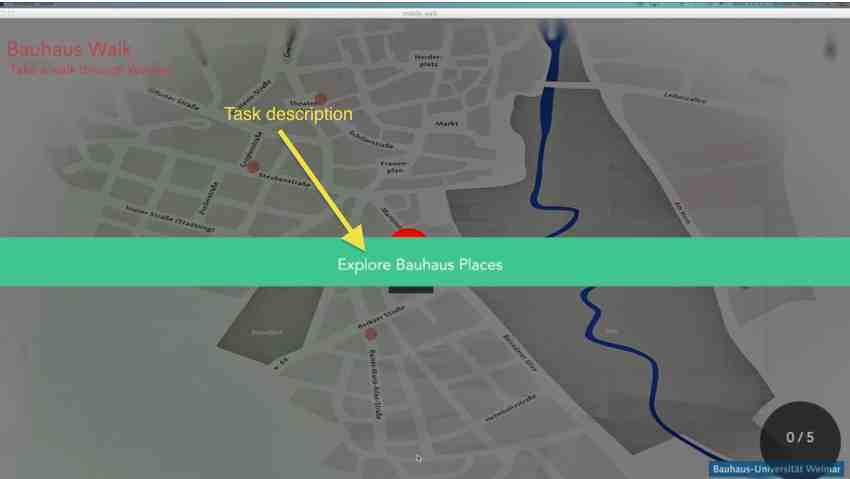
\includegraphics[width=\textwidth,height=4cm]{Figures/6/mobile/task_desc}
        \caption{Task description}
        \label{fig:task_mobile}
    \end{subfigure}
    \caption{Transitions of interfaces.}
    \label{fig:Switching_between_phases_mobile}
\end{figure}


\item Interation interface \\
The second screen is the interaction screen for the participants. The participants can navigate the cursor using their phone controller page. It can be seen in the below picture, the user is controlling the cursor and has explored one location. The user's defined name is also shown on the cursor so that the user do not lose track of his/her cursor. A small circle around the target location is shown is to determine the area of intersection. The interaction completes when all the locations are explored or the interaction time has finished.

\begin{figure}[H]
    \centering
    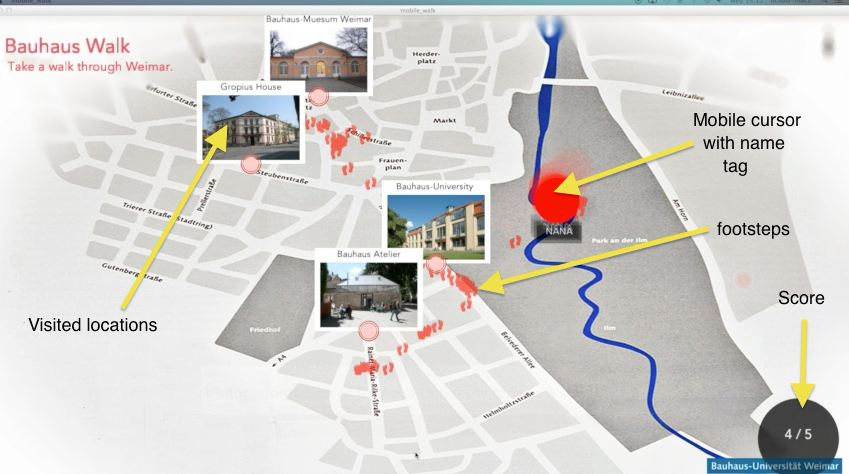
\includegraphics[width=120mm,height=70mm]{Figures/6/mobile/interaction_inter}
    \caption{Mobile interactive interface}%
    \label{fig:mobile_secondinterface}%
\end{figure}



\item Mobile interface: \\
This interface was designed by a student project called \emph{MMM Ball} \cite{MMMball, MMMball2} in Bauhaus University.
When the user opens the webpage and enters his/her name, the below interface would appear. The interface is simply designed and has two elements, the cursor and the select button. With cursor the user can navigate inside the map to reach target locations and then presses the select button to explore that location.

\begin{figure}[H]
    \centering
    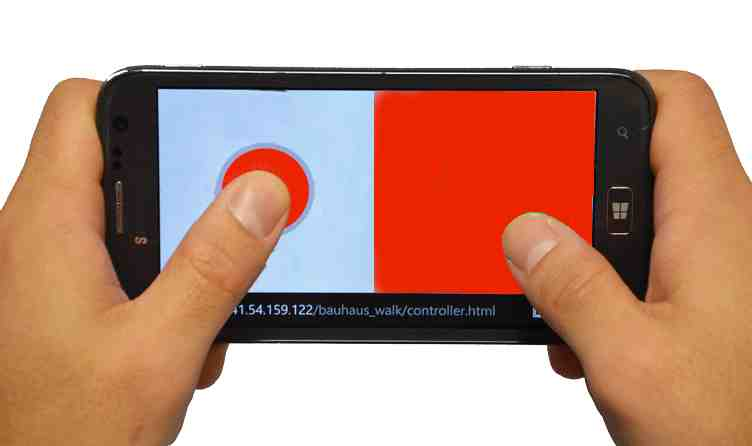
\includegraphics[width=100mm,height=60mm]{Figures/6/mobile/mobile_interface}
    \caption{Mobile controller interface: The left side is the cursor and the right side is the select button.}%
    \label{fig:mobile_controllerinterface}%
\end{figure}


\end{enumerate}

\section{Research questions}

\begin{enumerate}
\item   How fast do users understand \emph{Call-to-Action}?
\item   How fast participants react to the \emph{Call-to-Action}?
\item   How easy it is for the participants to understand the interaction task?
\item   How long does it take for the participants to complete the interaction or visit all the target locations?
\item   What are the major usability flaws that prevent users from advertisement interactions?
\item   What is the difference between mobile and body performance?
\item   How the applications would perform in single user interaction and in multi user interaction?

\end{enumerate}

\subsection{Video advertisement}
\begin{enumerate}
\item   Do participants understand the content of the advertisement?
\item   How many elements of display can participants recall after their first interaction?
\end{enumerate}


\section{Test Design}
This study used a within subject design, in which each participants were asked to experience with both body and mobile prototypes. The interaction sequence was interchanged for participants in order to counterbalance the learning effect.

\subsection {Participants}
12 participants were invited for the usability testing, from which five participants were female and seven were male. Most of the participants had computer science background and were familiar with mobile and had seen or worked with body sensing technologies. All participants were familiar with QR code except one participant. 

\subsection{Task}
Participants were not told about any specific task, they were asked to explore the system by their own and understand the task. To avoid different outcomes participants were told to continue interaction until they encounter back with the first stage of the application. So the tasks for participants were to start from the initial stage of the interaction (body /mobile) and continue until they reach the initial stage again.

For body interaction, no extra device was required to accomplish the task, but for the mobile interaction a mobile phone was required. The participants were not told that the use of mobile is required unless they tried to use their own phone or asked for it from me.


\begin{itemize}

\item \textbf{Task understandability:} \\
Participants were told to \emph{Think-Aloud} on what task will they perform at each stage. 


\item \textbf{Performance measurment:} 
\begin{itemize}
\item \emph{Call-to-Action} understanding duration \\
The time from when the user saw his/her silhouette until he/she understood / approached to start the interaction. For body \emph{Call-to-Action}, this duration is measured if the person intentionally moved toward the screen, and for mobile \emph{Call-to-Action}, when the person pulled the phone out.

\item Triggering game duration\\
This time is measured from the time the user understood how to start the interaction until the user actually starts the interaction. For example, in case of mobile interaction, the time is measured from the time the user takes out the mobile until he logins and opens the interaction controller.

\item Task understanding duration \\
This time is measured when the user starts the game until he/she understands the interaction task.

\item Task completion duration \\
Task completion time is measured from the time interaction starts until the interaction ends. 

\end{itemize}


\item \textbf{Content recall:} \\
After the first interaction with the advertisement, participants were immediately given a paper and a pen to write down the name of anything that they could recall. The interactions (mobile and body) were counterbalanced between the participants.

\item \textbf{Usability issues:} \\
Each participant was given five minutes to interact with both the mobile and the body advertisements. Then follow up questions were asked regarding the issues they faced. The usability issues like (confusing, unclear events and mistakes) were observed by the moderator at the scene and later while watching the recorded videos. 



\end{itemize}

\subsection{Data Gathering }
The below data were gathered.

\begin{itemize}

\item Performance data: \\
 The performance data of participants like, \emph{Triggering game duration}, \emph{Task understanding duration}, \emph{Task completion duration} and \emph{Whole interaction duration}was collected from both mobile and body interactions. To get an overview of performance in general the mean duration of the performance data were computed.

\item Preference data: \\
The preference data is the measures of participant opinion or thought process. The below preference data were collected.

\begin{itemize}

\item \emph{Think-Aloud} quotes \\
These quotes were noted during the video observation. These quotes were important to check at which time users understand about the interaction and tasks. 
It also helped to analyze their reaction and feedbacks toward the tasks being done.

\item Interview transcripts \\
All the interviews were transcribed and color-coding technique was applied to analyze and comprehend different aspects and categories from the defined questions.


\item Recordings \\
There were two different recordings done during the session, first was video recording using camera at the back of the room, that could record user actions and the computer screen and the second recording was the screen recoding of the application using \emph{QuickTIme} screen recorder. These recordings were used to analyze behavior, application performance and listen to the things participants said during interaction.


\end{itemize}



\begin{figure}[H]
    \centering
    \begin{subfigure}[H]{0.45\textwidth}
        \centering
        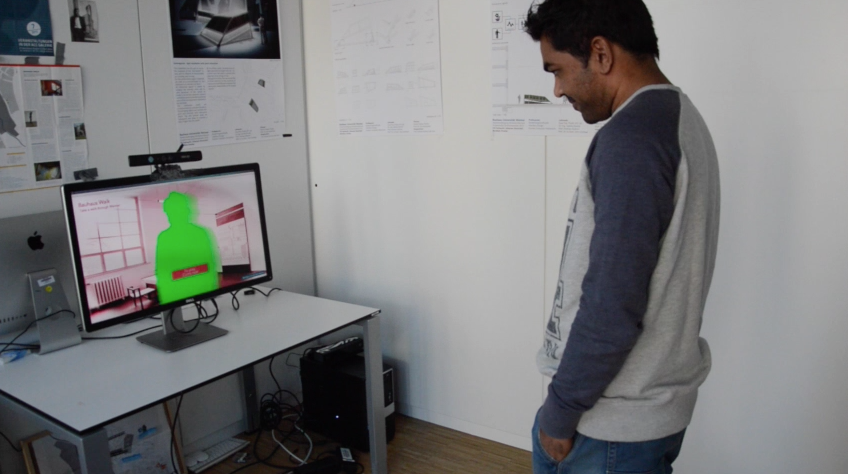
\includegraphics[width=\textwidth,height=4cm]{Figures/6/singleBody}
        \caption{Participant in body interaction mode.}
        \label{fig:singlebody}
    \end{subfigure}
    \begin{subfigure}[H]{0.45\textwidth}
        \centering
        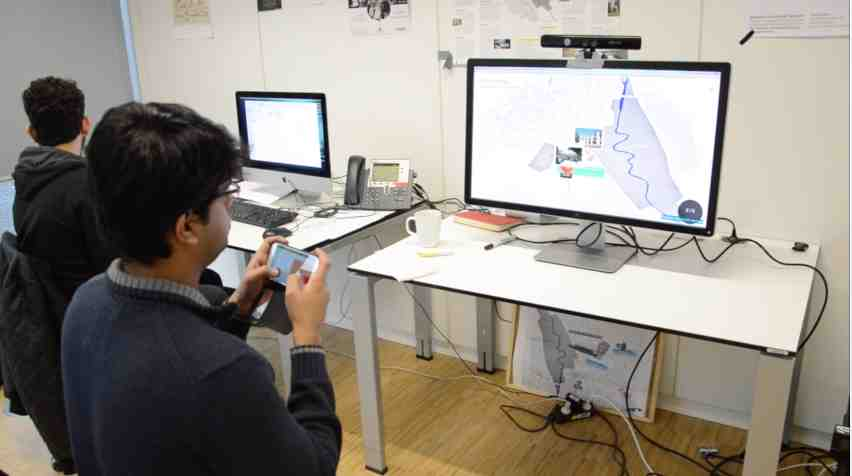
\includegraphics[width=\textwidth,height=4cm]{Figures/6/singleMobile}
        \caption{Participant in mobile interaction mode}
        \label{fig:singleMobile}
    \end{subfigure}
    \caption{Participant's video recordings}
    \label{fig:Focus_group_room}
\end{figure}

\end{itemize}



\section{Findings}


\subsection{User performance}


\begin{itemize}

\item Mobile Interaction performance: \\
The chart shown below exhibits the performance data, when the participants used the mobile interaction.
The y-axis shows duration in seconds and x-axis shows the phases(aspects). You can see performance chart for each individual of mobile in Appendix \ref{app:mobile_performance}.




\begin{figure}[H]
\centering
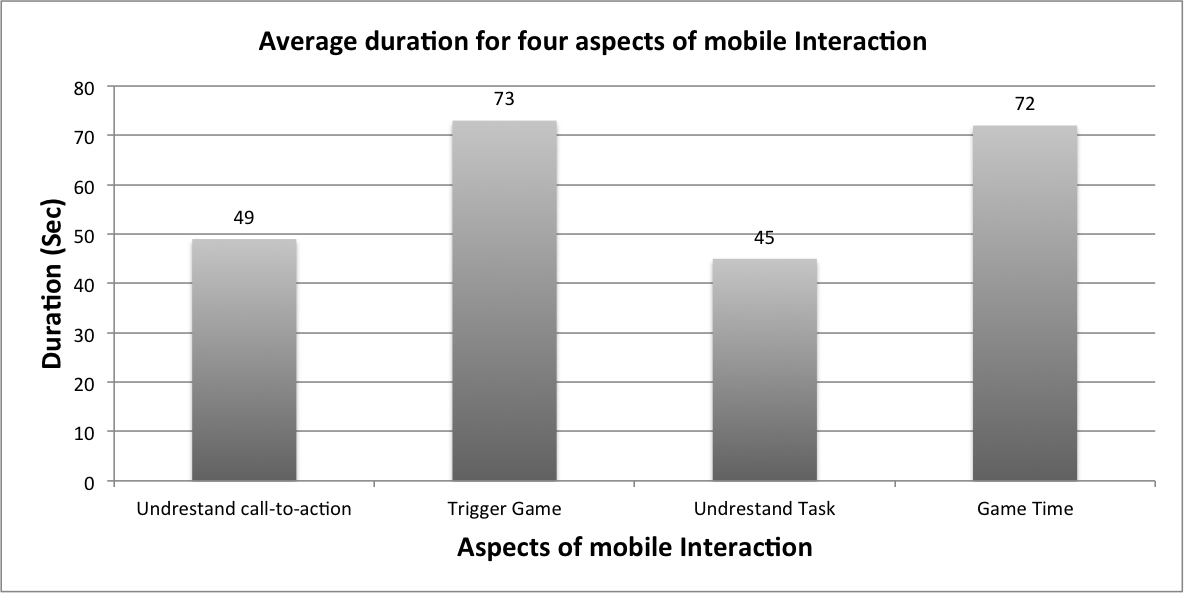
\includegraphics[width=12cm,height=5cm]{Figures/6/mobile_average}%
 \caption{Chart that shows each aspect with respect to duration. }%
 \label{fig:mobile_average}%
\end{figure}

Participants took 49 seconds in average to understand \emph{Call-to-Action}. After participants understood what to do, it took 73 seconds in average to trigger the game (\emph{Triggering game duration}). It took 45 seconds in average to figure out how to do the task (\emph{Task understanding duration}) and 72 seconds to complete the task(\emph{Task completion duration}). As a result in average 240 seconds were taken for whole interaction time.
%
%\begin{figure}[H]
%\centering
%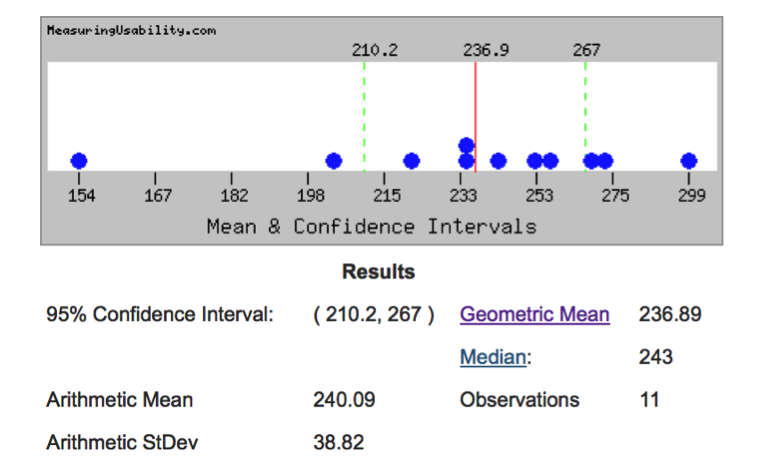
\includegraphics[width=12cm,height=6cm]{Figures/6/mobile_mean}%
% \caption{Confidence interval for Mobile interaction all phases duration }%
% \label{fig:mobile_mean}%
%\end{figure}

%above chart is generated in an online tool [1] with a confidence interval up to 95\% for complete interaction time for all 11 participants; the confidence interval is between (210.2, 267) the chart shows the Arithmetic standard deviation to be up to 38.82 seconds, Arithmetic Mean to be 240 seconds

\item Body Interaction performance: \\
The chart shown below exhibits the performance data, when the participants used the body interaction.
The y-axis shows duration in seconds and x-axis shows the phases(aspects). You can see performance chart for each individual of mobile in Appendix \ref{app:body_performance}.

\begin{figure}[H]
\centering
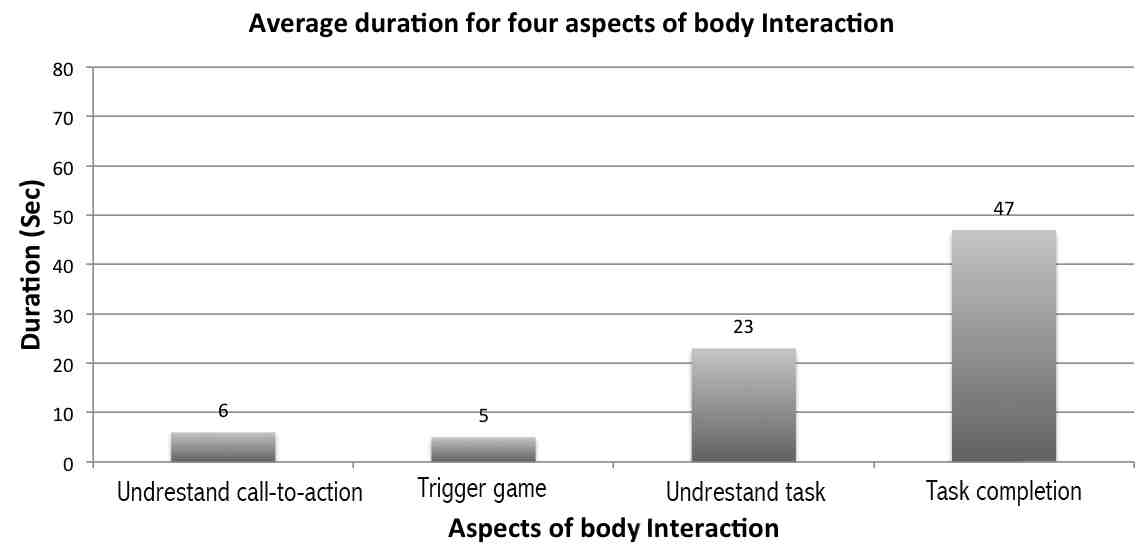
\includegraphics[width=12cm,height=5cm]{Figures/6/body_average}%
 \caption{Chart that shows each aspect with respect to duration}%
 \label{fig:body_average}%
\end{figure}

As can be seen above most of the participants finished the whole interaction in approximately 81 seconds, which is much better than mobile interaction. It took 6 seconds to understand \emph{Call-to-Action}. It took 5 seconds to trigger the interaction and start the game(\emph{Triggering game duration}). Participants took 23 seconds in average to understand the task (\emph{Task understanding duration}). And it took 47 seconds to complete the tasks(\emph{Task completion duration}).
%\begin{figure}[H]
%\centering
%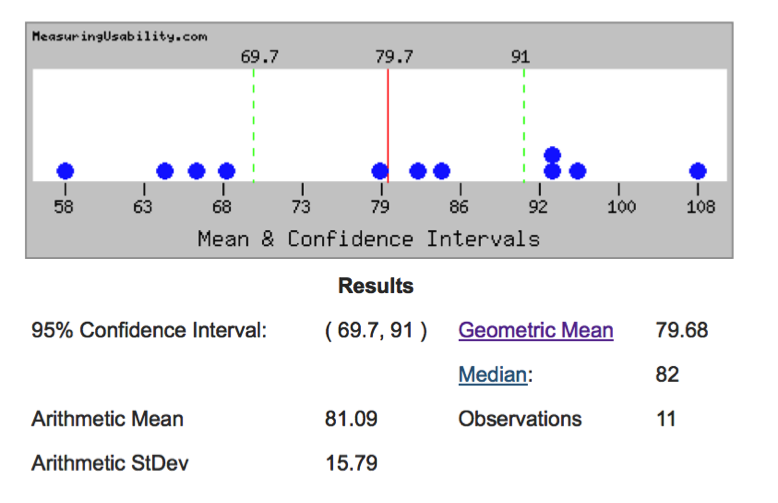
\includegraphics[width=12cm,height=6cm]{Figures/6/body_mean}%
% \caption{Confidence interval for body interaction all phases duration }%
% \label{fig:body_mean}%
%\end{figure}

%The above confidence interval for body interaction is generated using the web tool [1] for whole body interaction time. In which with the confidence interval of 95\% is between (69.7 ? 91) seconds, with the standard deviation of 15.79 seconds.


\item Body Vs. Mobile performance: \\
The following graph shows that the body interaction is much better than the mobile interaction in terms of performance. The whole interaction time of body is less than the half of the time of mobile interaction. 

\begin{figure}[H]
\centering
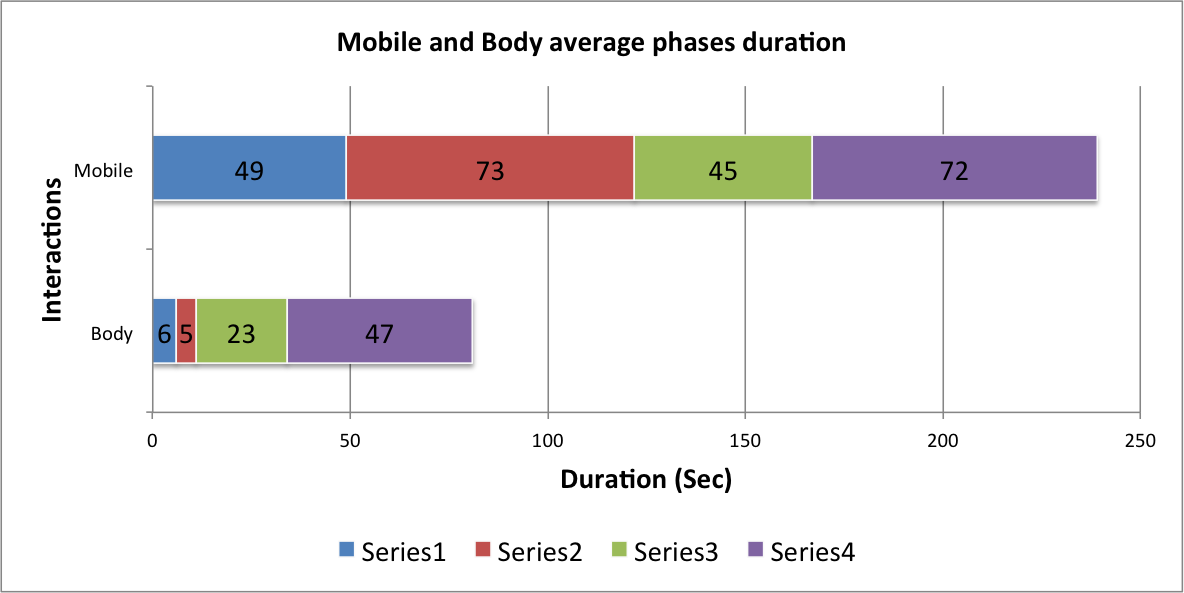
\includegraphics[width=12cm,height=6cm]{Figures/6/mobile_body_performance}%
 \caption{Comparison of body and mobile interaction performance }%
 \label{fig:mobile_body_performance}%
\end{figure}

81 second was the mean value of the all the participants’ performance with body interaction and 240 seconds is the mean value of the same participants with mobile interaction. The following chart shows other comparison of each aspect as described.


\begin{figure}[H]
\centering
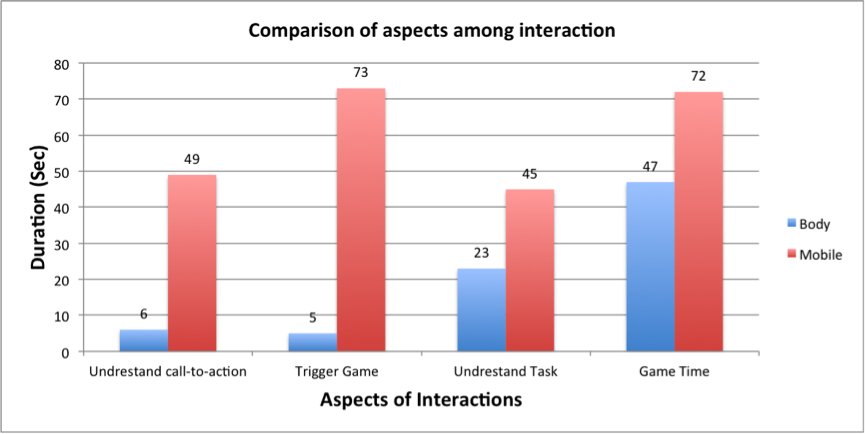
\includegraphics[width=12cm,height=6cm]{Figures/6/mobile_body_aspect}%
 \caption{Comparison of the aspects of interaction among body and mobile }%
 \label{fig:mobile_body_aspect}%
\end{figure}


The mobile interaction took much longer than body interaction for each phase or aspects, as \emph{ANOVA} revealed a strong significant difference of \emph{Call-to-Action} between body and mobile interaction ( \emph{(F1,11)=22.4758, p < .001 (p=.0001)}). A post-hoc Tukey test shows that participants understood very quickly the \emph{Call-to-Action} of body interaction compared to mobile interaction technique.

\emph{ANOVA} revealed a significant difference of triggering game between body and mobile interaction, ( \emph{(F1,11)=124.1066, p < .001}). Post-hoc Tukey test shows that in body interaction the triggering happens much faster than mobile interaction. 

\emph{ANOVA} revealed a significant difference of task understandability between body and mobile, ( \emph{(F1,11)=7.1340, p < .05 (p=.0147)}). A post-hoc Tukey test shows that participants understood the task very faster compared to mobile technique.

Interaction time was also significantly different as \emph{ANOVA} test strongly suggested a significant difference between the mobile and body interactions, ( \emph{(F1,11)=19.7000, p < .001 (p=.01)}). Post-hoc Tukey test strongly states that body interaction takes less time to complete the interaction compared to mobile.

\end{itemize}



\subsection{Usability issues}
The following usability issues are gathered from participant while observing them during the interactions.


\begin{itemize}

\item \textbf{Mobile Interaction:}
\begin{enumerate}
\item	Call-to-Action
\begin{enumerate}
\item At the first look of application, most participants did not read the text on the screen, they were expecting other way to get quick information. But after many tries with their body, they had to read the information text. 

\item   Participants did not understand about the phone icon or the browser animation on top of it until they figured by themselves.
\item   Frustration of typing the IP address.
\item   The size of QR code was small.
\end{enumerate}


\item   Use of mobile phone.
\begin{enumerate}
\item   In the beginning the participants did not except to use their own phone for the interactions; Many times participants asked, ``\emph{Should I use my phone?}'' 
\item   Most participants did not read the instruction to tilt their phone and even if they accidently had tilted the phone.
\item   There was no instruction to turn-on the tilt-sensor in the mobile phone.
\end{enumerate}

\item   Login page
\begin{enumerate}
\item   Some of the participants were confused with the word Login. Participants thought that they would have to provide some sort of username and password to the system, and one participant reacted to this strictly and refused to login to the webpage using his phone.
\end{enumerate}

\item   Task description
\begin{enumerate}
\item   The task description was shown after the participants login to the system despite of whether the phone is tilted or not, most participants missed to read the task description because they were busy with their phone to tilt it and by that time the description on the screen was gone.
\end{enumerate}

\item   Controller
\begin{enumerate}
\item   Participants did not read and saw the instructions for phone.   
\item   Many participants complained about the elasticity (automatic centering feature) of cursor. They had to reposition the cursor for another location to explore.
\end{enumerate}
\end{enumerate}


\item \textbf{Body Interaction:}

\begin{enumerate}
\item   \emph{Call-To-Action} \\
The silhouette was projected with largest scale for attraction attention, but the silhouette scales down and adjusts to person position (x, z) on the display. When users triggered the interaction by coming close to the screen, then participants could not see themselves because the mini-silhouette would adjust outside at top of the display. If participant moved back then they could see the silhouette back. 

\item   Silhouette controlle \\
There was no instructions on how to move the body physically to perform the tasks. But participants tried for themselves to find a way to interact.

\item   Alert image \\
Alert image that shows a Hands-Up person lead to confusion at the moment where users were much closer to the system.
\end{enumerate}

\item Advertisement video: \\
\begin{enumerate}
\item The slides were switching fast.
\item Some did not like the colors and theme. 
\end{enumerate}


\end{itemize}

\subsection{Advertisement goal}


\begin{itemize}


\item Do participants understand the content of the advertisement?\\
The criteria for recalling the advertisement was that participants should recall ``\emph{Bauhaus-Walk}'' word and explain what does it do. They could also explain if the interaction technique gave them an idea what could be the advertisement about. At best users can recall the date, timing and location of the tour program. The findings for these criteria are listed below.

\begin{enumerate}

\item   \textbf{Ad goal description} \\
To find out ad goal description, what all participants experienced with the very first interaction technique, were immediately asked about the goal of the advertisement. I wanted to know if the participants would understand about the advertisement on their very first try. All of the participants were speaking in English language.  The entire participants responded as they finished the interaction. 9 participants accurately described the goal of the advertisement, but 2 participants generally described the goal because at the beginning the advertisement video was in German language.

\item   \textbf{Ad-related elements recalled}  \\ 
After the participants described the goal, they were given a piece of sheet to draw and write any element related to the interaction and advertisement with in five minutes. All the sketches drawn and keywords written by the participants were manually counted. The count is in the following diagram. 


\begin{figure}[H]
\centering
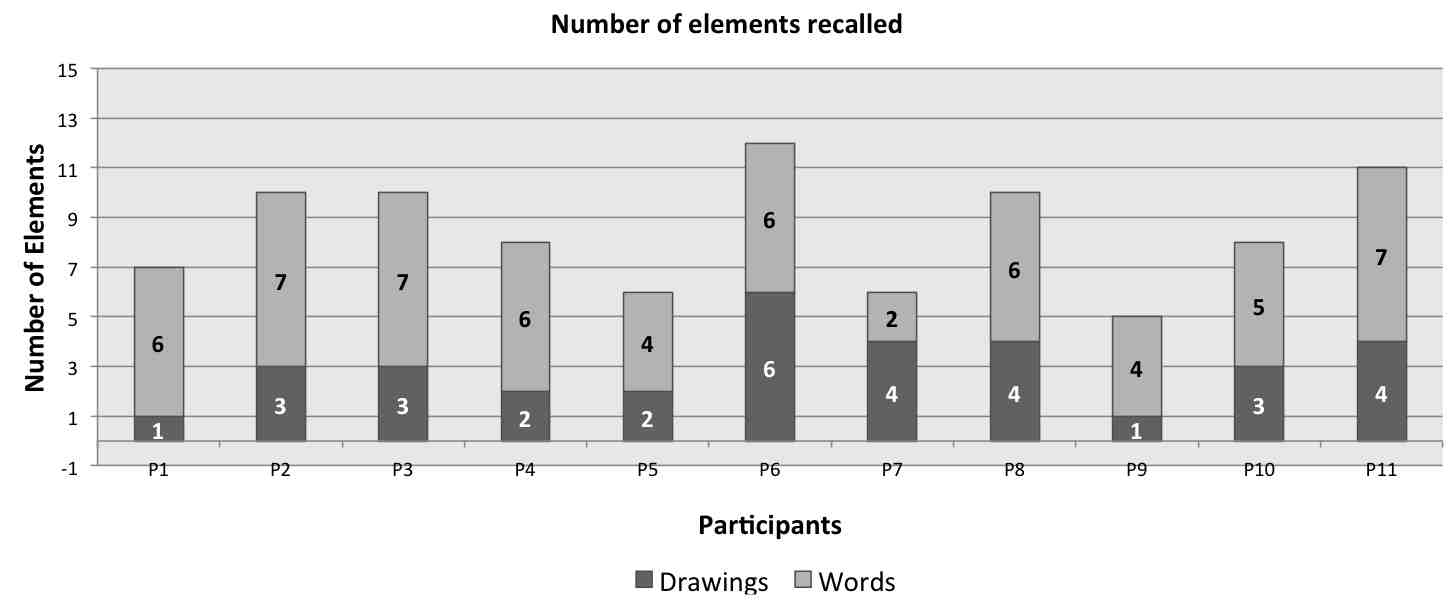
\includegraphics[width=0.9\textwidth,height=8cm]{Figures/6/word_recall}%
 \caption{Number of words and drawings of the advertisement elements }%
 \label{fig:word_recall}%
\end{figure}

\end{enumerate}

\item Word cloud (Wordle): \\
All the keywords written by the participants were collected in one text file and visualized in word cloud technique by using an online tool \emph{Wordle}\footnote{Wordle: \url{http://www.wordle.net/create}, last accessed: 10 May 2016} .
The word cloud visualizes most key words that had high frequencies. Those keywords are the ones actually related to the advertisement, it seems most location names that participants interacted with are recalled a lot like, ``\emph{Bauhaus University}'' ,``\emph{Haus-am-horn}''and others. The program name ``\emph{Bauhaus-Walk}'' is also in high frequency list, and even the day of the event is mentioned too.


\begin{figure}[H]
\centering
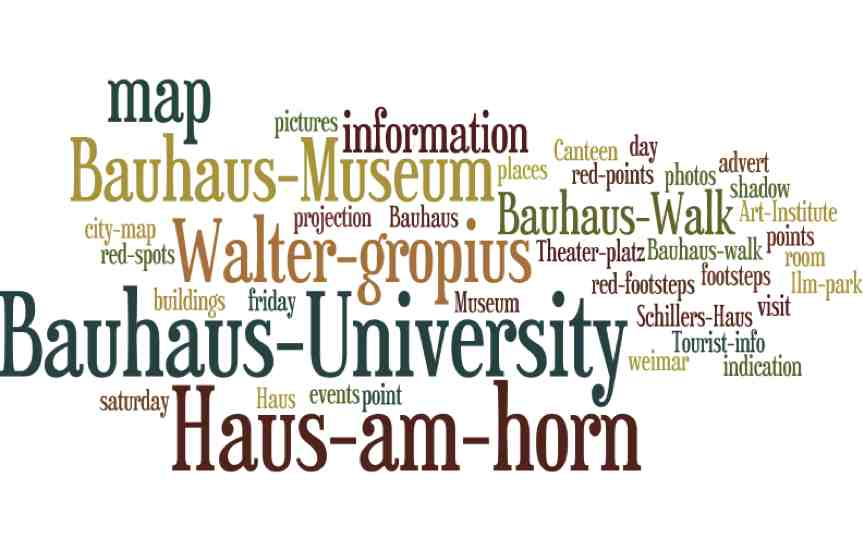
\includegraphics[width=0.8\textwidth,height=8cm]{Figures/6/wordle}%
 \caption{Word cloud representation of the keywords}%
 \label{fig:wordle}%
\end{figure}


\end{itemize}

\subsection{Interview Findings}
All the interviews transcripts were coded for better analyzing, appropriate connections to categories were found and these categories are shown as a diagram.

\begin{itemize}

\item \textbf{Mobile Categories:} \\
Many important categories were created from the responder's codes, see Appendix \ref{app:mobileinterviewcodes_} for the diagram. These categories reflect the functionality, nature, issues and complications of the mobile interaction technique. Most of them point out negative concerns and some positive feedbacks too about the interactions, which is discussed below.

\begin{enumerate}
\item	Comfortable: \\
	Mobile interaction is comfortable in the context of public environment, users do not feel shy to work with their phone, they have more privacy as one user said ``\emph{I think for people moving in public could be more embarrassing if you just use your phone the people passing by will not pay attention}''. Users can also work with the display from a far location rather than standing in front of as one participant said, ``\emph{you can comfortably set far away see the screen and start interacting}''.
\item	Activity: \\
	This method has less Activity, participants do not have to move their body to reach certain points in the map, instead they can use their phone and stand or sit steady. With the tip of their finger can easily explore locations, as one of the user said ``\emph{I could go with the tip of my finger and it helped me all the places I visited}''.
\item	Dependency:\\
	On the other hand, this interaction is dependent on many things obviously a mobile phone, if the user does not have a mobile phone the interaction cannot happen, a participant asked, ``\emph{How would I have played if I have not brought my mobile phone?}'' Another dependency is the WIFI connection, one participant pointed out ``\emph{And then the fact that I had to be connected to a WIFI, that was because I did not understand do we have to be in the same Internet (Network)?}'' 

\item	Complicated:\\
The process seemed complicated for instance, entering the IP-Address or scanning the QR-code. Further reading the instructions, logging in with a name, tilting the phone and finally interacting with the controller elements such as the button and the cursor. Most of the participants complained about regarding this by stating, ``\emph{Because it is a headache for me to take out my phone and use all this login, and waste my time.}'' another commented like ``\emph{for exploring you have to push that red button, that was a bit confusing.}''


\item	Annoying:\\
One of the annoying things pointed out by the participant was that the QR-Code was being covered by the person's silhouette, who was standing in front of the display, the user said, ``\emph{QR-Code was small and when I was coming near the screen to scan the code, my body was covering it}''.

\item	Clarity:\\
There were many instructions like Access-information, mobile instruction and task instruction, but these instructions was also not clear to them as one of the participant mentioned, ``\emph{that controller was also not clear, because I though the red areas is the touch area that I can scroll and the red button was a click}'' another participant replied like ``\emph{there were very few descriptions, I guess the word login was miss-phrased, it was not really a login it was just chose a name}''. Another participant was not sure whether to use mobile phone or the screen has touch capability as he replied ``\emph{at first I saw the map, and there were points on the top first I tried to touch}''.


\end{enumerate}


\item \textbf{Body Categories:} \\
Body interaction was more appreciated by the participants. From the interview transcripts an intensive color code categories were derived, see Appendix \ref{app:bodyinterviewcodes_} for the code diagram. The following positive and negative opinions were derived and categorized. 

\begin{enumerate}
\item	Enjoyment:\\
Participants had the sense of enjoyment and fun, as one of participants said, ``\emph{I liked the second one because it seemed more involving and I think it was more fun}'', another user said ``\emph{I liked this interaction; it was more good and fun.}'' , 

\item	Easy:\\
Users found the interaction to be very easy, simple and smooth, a user said, ``\emph{The body movement was good it was smooth}'' another user said, ``\emph{It was much easier than the previous one, it was much better, umm it was not confusing}''. The call-to-Action seemed much easier, one user said, ``\emph{I saw saying me to come near, and when I came the game started, that was very easy to use}'', and the interaction with the game elements was also easy to understand, one participants said ``\emph{it was easy to come near to the screen and first I did not understand how to play the game but when I saw my avatar that is moving with me then I realized and did the tasks}''

\item	Immersion:\\
Some participants said they were some how immersed with the game, like one said, ``\emph{I felt that I was really part of it}'', another said, ``\emph{With the body you look your own avatar in the map and you feel that you are in the map.}''

\item	Engaging:\\
The body technique seemed very engaging and users wanted to play more and more, one said, ``\emph{It is so engaging and it is like that it needs you}'', another said, ``\emph{it is like you want to put the footsteps exactly on the street}'' , ``\emph{it seemed more involving}''. 

\item	Issues:\\
On the other hand, the body interaction also had some issues, like one of the participants pointed out that the interaction would be difficult if it is in crowded area. One said, ``\emph{If two people interact then they can crash at each other}''. Participants complained about physical space ``\emph{I felt was the space there was not enough space in here}''. Bad tracking of the body and unexpected locations were triggered by fast movement, one participants said, ``\emph{I guess the application was tracking me really bad}'', ``\emph{when I was moving to some areas fast suddenly that point was being triggered.}''

\item	Embarrassing:\\
Some participants said that they would not try the application at public space because it could be shame or embarrassment for themselves, ``\emph{moving in public could be more embarrassing}''

\item	Confusion:\\
The projection of silhouette on the advertisement also made some participants get confused and that it was also distractive, like one said, ``\emph{I saw my silhouette at the last time I was playing, because I was curious that why is it there}''. 

\end{enumerate}


\item \textbf{Others:}

\begin{enumerate}
\item	\textbf{Interface}\\
The interface was appreciated by all the participants, as one said, ``\emph{I really liked the map}'', another user said, ``\emph{the footsteps were cute}''.

\item	\textbf{Non-controllability}\\
The flow of the interaction was also observed by the users, which they found annoying. As a participant stated that ``\emph{I do not want to be forced to see all the places and then see the advertisement}''. The video advertisement was also not in control a user said, ``\emph{There was nothing to answer, it gave me the impression that okay; this was an advertisement someone did it and I could not change the flow of it.}'' 

\item	\textbf{Distraction}\\
The projection of the silhouette after the interaction body or mobile technique was a distraction factor, because participants would not notice the video advertisement but would notice themselves. 

\item	\textbf{Speed}\\
The pictures for the locations and the advertisement video were fast, a user said, ``\emph{The description of the places were very fast, when I was trying to read it, it disappeared.}'', 
\end{enumerate}

\end{itemize}


\subsection{Application Performance}
It did not crash or hang in the middle of the interaction, but during the multi-user interaction, the application faced some delay in both the body and the mobile interaction due to many participants (5-7) engaging at the same time. Changing the JRE version from 32bit to 64bit solved this issue, and along with this the processing version was also changed from 32bit to 64bit. The usage memory was increased to its maximum for better processing.

\begin{figure}[H]
    \centering
    \begin{subfigure}[H]{0.45\textwidth}
        \centering
        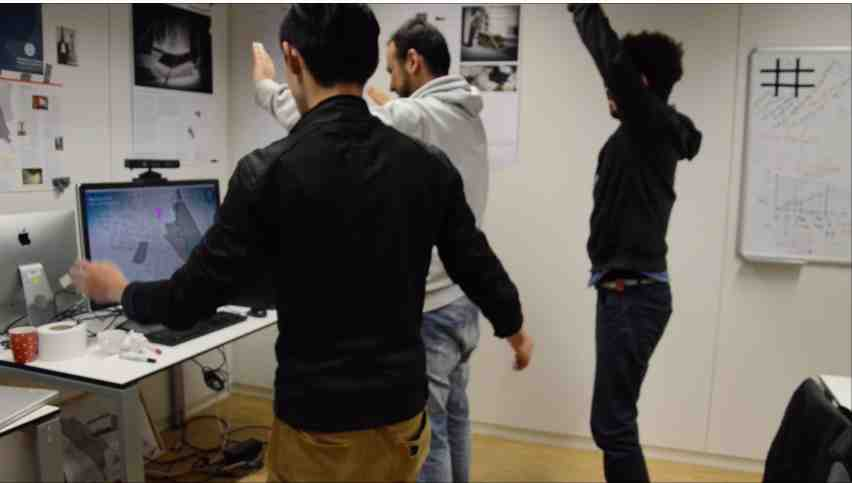
\includegraphics[width=\textwidth,height=4cm]{Figures/6/groupBody}
        \caption{Group body interaction.}
        \label{fig:groupbody}
    \end{subfigure}
    \begin{subfigure}[H]{0.45\textwidth}
        \centering
        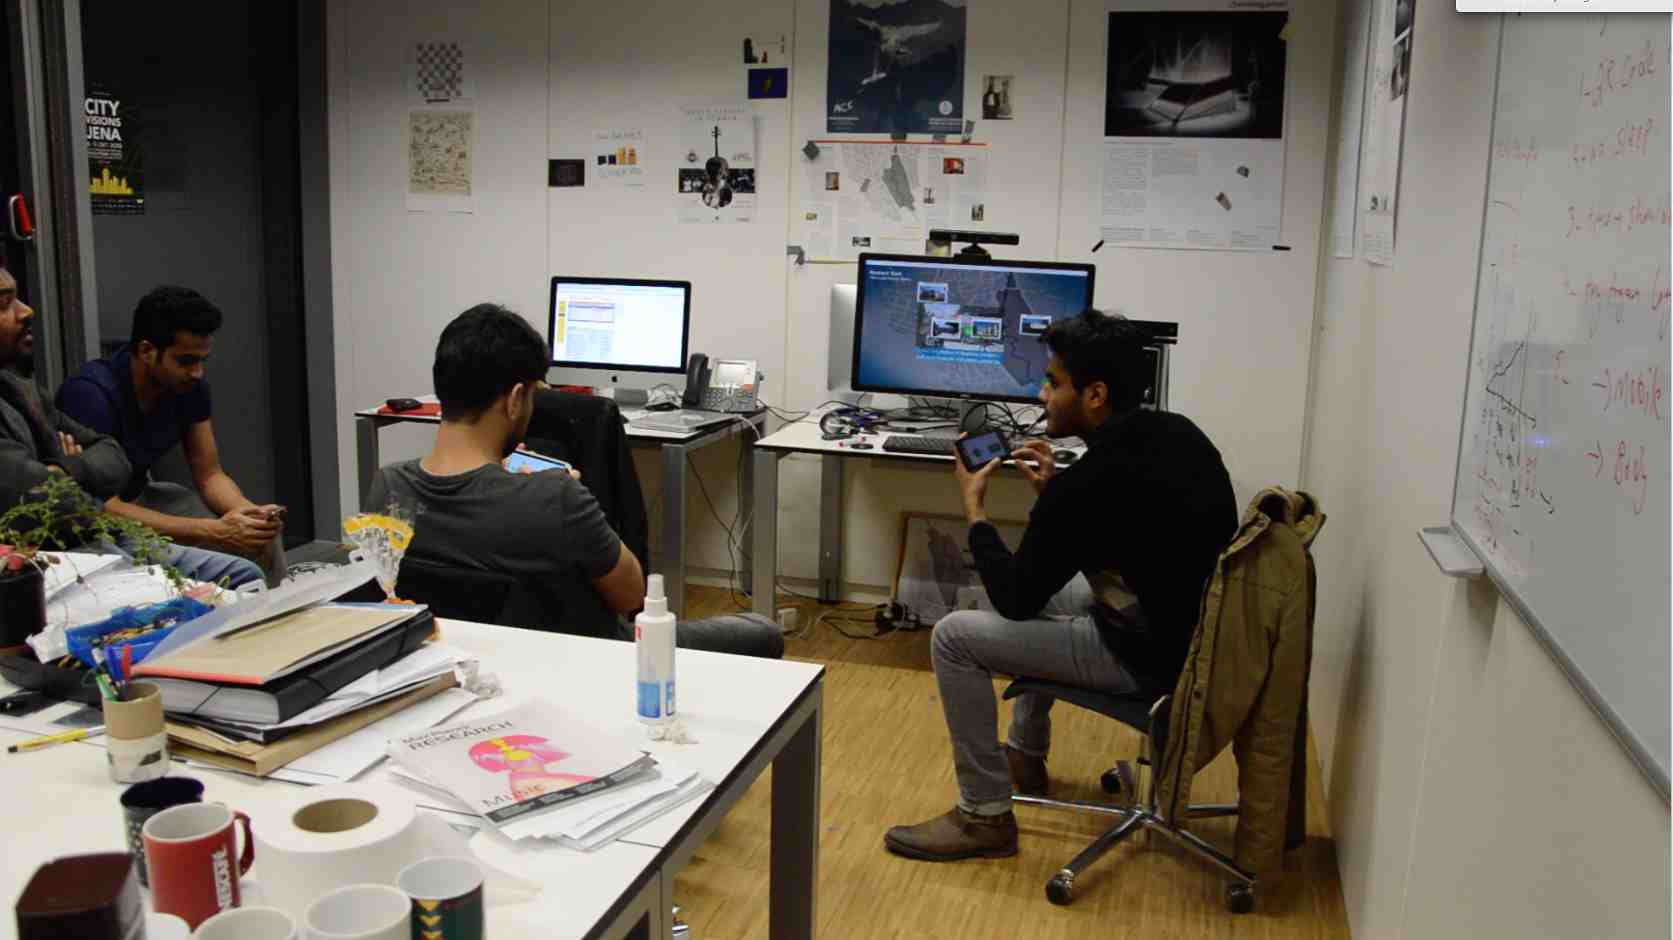
\includegraphics[width=\textwidth,height=4cm]{Figures/6/groupMobile}
        \caption{Group mobile interaction.}
        \label{fig:groupmobile}
    \end{subfigure}
    \caption{}
    \label{fig:Focus_group_room_interactive}
\end{figure}


\section{Discussions}

The performance \emph{Call-to-Action} (``To play come near'')of the body interaction was better than the mobile \emph{Call-to-Action}(Connect to Wi-Fi, Login and open controller) because of many reasons, (1) \emph{Understandable:} The sentence was clear and comprehendible for the participants,  (2) \emph{Natural to perform:} The action of walking is completely natural and easy to perform. But the mobile \emph{Call-to-Action} seemed to be complicated and time consuming because of many preseasons. (1) \emph{A lot of info text}, There were many text on the screen for the participant to read and understand before interaction starts. (2) \emph{Text size}, the texts size was small and participants could not read if standing in distant to the screen. (3) \emph{occlusion of text}, the text was occluded by the silhouette an when the participant wanted to get closer more area of the text was being covered. The users had to stay at side of display to read the information text. 

Additionally, not all mobile phones have the tilting sensor enabled, which resulted to stop users from opening the controller. Participants were forced by application to enable the tilt sensor of their phone then open the controller. This extra task is in fact annoying and time consuming. 

The average time for performing the interaction in body interaction was also significant faster than the mobile interaction. One of the reasons could be the live silhouette representation of the participant on the city map, which gave the clue of walking and exploring locations. But in mobile interaction the cursor representation was not obvious to the users, participants had to try to find they way of interaction.  

Beside the body and mobile interaction usability issues, still the participants could understand the goal of advertisement. Here I list the key factors for advertisement understanding:
\begin{enumerate}
\item   \textbf{Game environment} \\
The game environment designed for the interactions had a major impact for understanding the advertisement goal. For example one of the participants replied ``\emph{I saw a map and different places, so I guess touristic places that I can visit in Weimar.}''. Besides the map, there were blinking points on the map, on which most people are familiar with, showing the interest regions of the city. One of the participants replier,  ``\emph{ I think it was about tourist places in the city, at first I saw the map, and there were points on the top}''. Participants already linked the points with the touristic places of Weimar automatically. 

\item   \textbf{Interaction technique} \\
In the body interaction, where walking is involved, participants got a clue about the advertisement indirectly only by walking and linked walking as visiting locations. Like one of the participants replied ``\emph{Discovering Weimar. The Bauhaus-Walk. It was the advertisement about those locations that the people can visit in the tour.}''. It is very fascinating to read that answer from which the whole goal of the advertisement can be derived.

\item   \textbf{Advertisement video} \\
The advertisement video had an impact on the participants to be able to recall the advertisement, one of the participants replied that ``\emph{I saw many pictures coming about Bauhaus and the program times and day}'', though that the users understood a little about the advertisement they also complained about the video for being fast.
\end{enumerate}


\section{Conclusion}
This chapter concludes that users performed better in the body interaction than the mobile interaction technique. Participants preferred the use of body interaction than mobile in public environment.

Body interaction was more natural and convenient for participants. This interaction had no dependency to any preferable device like mobile phone. The \emph{Call-to-Action} was very understandable and performing of the action was very natural. Body representation on the map provided a strong clue of ``\emph{walking}'', this clue had two major benefits, (1) understanding the task and performing it. (2) Understanding the goal of the interactive advertisement. Participants felt enjoyment and immersion while interacting using their body. Despite the positive feedbacks, there were some usability issues like incorrect mapping of the silhouette when the user was standing near, not implementing alert messages, and also facing interaction difficulties if there were multi-user because the users were colliding to each other. On the whole, the overall performance and acceptability of this technique was very convincing compared to mobile interaction.


The mobile interaction had various usability issues and especially with the accessibility to the advertisement system. Participants took a long time to understand what was required to access because of unclear access-info text, unfamiliarity with QR code or phone icons, inserting name. Participants then took longer time to follow the steps to login to the system. Task completion time was also significantly low than body interaction.  Beside all these major issues two participants found it more comfortable to use it in public display because it will not cause the sense of embarrassment for them. While interaction it did not require more physical body movement but only required cursor movement. The participants also understood the goal of advertisement.

Considering the above issues, the next step would be to refine both prototypes and make it ready for evaluation on public space.
















